\documentclass[11pt]{article}
\usepackage{geometry}                % See geometry.pdf to learn the layout options. There are lots.
\geometry{letterpaper}                   % ... or a4paper or a5paper or ... 
%\geometry{landscape}                % Activate for for rotated page geometry
% \usepackage[parfill]{parskip}    % Activate to begin paragraphs with an empty line rather than an indent
\usepackage{graphicx}
\usepackage{amssymb}
\usepackage{epstopdf}
\usepackage{algpseudocode}
\usepackage{algorithm}
\DeclareGraphicsRule{.tif}{png}{.png}{`convert #1 `dirname #1`/`basename #1 .tif`.png}
\newcommand{\ttt}{\texttt}


\title{CS 5220 Project 2: Stage 1}
\date{}
\author{Elliot Cartee (evc34), Patrick Cao (pxc2), Ben Shulman (bgs53)}

\begin{document}
\maketitle

\section{Introduction}

For this project, our goal is to optimize a simulation of the shallow water equations with periodic boundary conditions. To accomplish this, we will use three main approaches:
\begin{itemize}
	\item Use profiling and vectorization reports to determine which parts of the code would benefit most from tuning
	\item Tune the serial code to maximize performance on a single core
	\item Implement domain decomposition so that our highly tuned serial code can be run in parallel.
\end{itemize}
We will then do scaling studies for our tuned parallel code to see how much we improve over the standard serial code, and compare our results to performance models.

\section{Profiling}

In order to identify what areas of the original \ttt{C++} code could receive benefits from tuning, we began with the standard profiling tool \textbf{Intel VTune Amplifier XE}. Using the profiler to identify which functions were slowest, we found that in the basic dam break example, the majority of time was spent in the following functions:
$$
\begin{tabular}{|c|c|}
	\hline
	function & time (seconds) \\
	\hline
	\ttt{limited\_derivs} & 1.323 \\
	\ttt{compute\_step} & 0.683 \\
	\ttt{compute\_fg\_speed} & 0.236 \\
	\hline
\end{tabular}
$$

We also found that no more than about $20$ milliseconds was spent in any other function.
Considering that these functions contain the vast majority of the computations, it is not surprising that they took the most time to complete.

We then profiled each of these functions individually to identify which parts were slowest. Unsurprisingly, we learned from profiling these functions that the steps which did real computation inside of \ttt{for} loops was the most expensive. Unfortunately we were unable to profile memory and cache accesses as the Haswell architecture on the chips we are using does not support much memory profiling via \textbf{VTune Amplifier}.

\section{Vectorization}

One of the key ways of improving performance is by maximizing instruction level parallelism through vectorization. In order to see what loops were and were not being vectorized, we began by looking at the vectorization reports generated by \ttt{ICC}. We found that none of the \ttt{C++} code was being vectorized due to assumed anti/flow dependencies in every \ttt{for} loop. Since we knew from profiling that the vast majority of time was spent in the functions \ttt{limited\_derivs}, \ttt{compute\_step}, and \ttt{compute\_fg\_speed}, we realized we could make large performance gains from vectorizing these functions as much as possible.

Our first attempt at improving vectorization was to resolve incorrectly assumed dependencies using \ttt{\#pragma ivdep}. This pragma tells the compiler to discount any assumed dependencies and only consider proven dependencies. This improves vectorization slightly for the \ttt{C++} code, but much of the code still does not get vectorized. Unfortunately, this vectorization sometimes led to only minor improvements, and was sometimes actually worse (in which case the compiler did not vectorize).

In an attempt to make vectorization more efficient we turned to Intel's vectorization guides, and found that the layout of the original data structure is not ideal\footnote{https://software.intel.com/en-us/articles/memory-layout-transformations}. The problem is that the the vector $u$ was originally stored as Vector of Arrays. Each array ($u$ cell) is length 3, thus making the memory structure of the vector $u$ be \ttt{[U0, U1, U2, U0, U1, U2, ...]}. Most of the computations in the slow parts of the code involve only a single dimension of $u$ at a time rather than using all 3 dimensions of each vector at the same time. This suggests that this Vectors of Arrays structure (VOA) can be improved by separating each vector into 3 vectors, one for each dimension, which allows unit stride access to different cells when working in the same dimension.

We implemented this method for each vector and found that while vectorization increased, overall performance actually decreased. This suggests that even though the VOA style did not seem like the best structure the compiler was still able to optimize better with the original VOA memory structure than the new memory structure.

Due to our struggles with vectorization in \ttt{C++} and the rewriting of the simulation code into \ttt{C} by Professor Bindel we decided to switch over to optimizing the new \ttt{C} code as it gives us more control over memory alignment, restriction, vectorization, etc. which \ttt{C++} made difficult. Further we are generally more comfortable with \ttt{C}.

\section{Domain Decomposition}

Given the local nature of the shallow water physics, this simulation is an ideal candidate for domain decomposition. Because calculating the water height and momentum at each cell depends only on nearby cells, this problem can be broken into subdomains, which processors can compute independently for several steps before needing to synchronize. In order to make implementing domain decomposition easier, we made some basic simplifying assumptions:

\begin{itemize}
	\item All simulations take place on a square grid of size $n \times n$.
	\item The number of processors $p$ is a perfect square.
	\item $n$ is divisible by $\sqrt{p}$
\end{itemize}

We will also use $b$ to refer to the batch size, meaning that $2b$ is the number of timesteps computed by each processor between synchronizations. (Note that we compute $2b$ instead of $b$ steps because of the grid offset in the Jiang-Tadmor central difference scheme being used).

For our implementation of domain decomposition, we maintained a global copy of the domain which is used to store the current state of the entire simulation. We then divide the domain into $p$ equally sized subdomains, with one processor being responsible for each. There were two approaches we considered for allowing each processor to compute the subdomain it was responsible for. The first approach is to keep only one copy of the whole domain and each processor will read and write to this shared memory. The second approach would be to have each processor maintain a copy of its subdomain and periodically synchronize up with the global copy of the domain. The first approach requires less copying of memory back and forth. However, since the subdomains overlap with each other, it requires us to guarantee thread safety for the shared global domain. The second approach requires more copying of memory but it can be done without needing to worry about thread safety. In addition to decreasing implementation complexity, the second approach is able to use the cache more efficiently. Since each subdomain will now be stored in a contiguous region of memory, this allows us to make more efficient use of spatial locality. 

Using this approach, we developed the following algorithm (written here in pseudocode):

\begin{algorithm}
\begin{algorithmic}[1]
\item Apply periodic boundary conditions to \ttt{domain}
\item Find $\ttt{max\_speed}$ in \ttt{domain}
\State $\ttt{dt} \gets 0.9*\ttt{cfl} / \ttt{max\_speed}$
\For {each processor}
	\State \ttt{subdomain} $\gets$ relevant part of \ttt{domain}
	\For {i = 1,2,...,b}
		\State \ttt{subdomain} $\gets$ \Call{compute\_step}{0} 
		\State \ttt{subdomain} $\gets$ \Call{compute\_step}{1}
	\EndFor
	\State \ttt{domain} $\gets$ \ttt{subdomain}
\EndFor
\end{algorithmic}
\end{algorithm}

We note that we have had to decrease the size of the time step $\ttt{dt}$ as we are now computing multiple time steps between each calculation of $\ttt{dt}$. While decreasing the time step increases the amount of computational time for simulations, decreasing the time step can lead to instability of the numerical method. Our current choice of $0.9$ times the CFL condition of $0.45$ is heuristic, and could very likely be improved.

\section{Offloading to The Phis}

Though the main processors on our cluster allow for high flop rate per thread, they do not support high parallelism as there are 24 possible threads per node. The shallow water simulation is ideal for a high level of parallelism due to the local nature of calculating the next timestep for each cell.

Offloading to a co-processor with a high number of threads (236 per node), makes sense when we are able to parallelize previously global computation such as the speed calculation for the entire simulation (see the previous section). Because of this there is no bottleneck where a single thread is solving a large problem on a single slow core of the co-processor. Finally, rather than having to move memory back and forth to do single large computations on the E5 processors and the highly parallelizable computations on the Phis, we can simply offload the entire problem to the Phis. This simplifies both the implementation of offloading and the potentially high latency costs that come with moving data between co-processors and the main processors.

Our implementation of offloading is rather simple, after generating the initial global simulation state, all work is passed off to the Phi accelerators. This works because all future work simply involves parallelizable work and the only data which needs to be copied over is the initial global simulation state, and some minor meta-data such as how long the simulation is to run for. The simulation is then run for its entirety by the Phi accelerator boards and then the results are copied back to the main processors memory for frame visualization, etc.

Though our implementation of offloading Phis involves only a single pragma to do all the work, it did require restructuring our code. For one offloading data to the phis which includes structs of pointers or arrays of pointers is complicated because the simple offload pragmas do not recursively follow pointers to copy all data each pointer points to.\footnote{https://software.intel.com/en-us/articles/effective-use-of-the-intel-compilers-offload-features} Thus naively this will result in accesses to invalid pointers which point to the Xeon E5 memory rather than the co-processor memory. To mitigate this problem we deconstructed all data passed to the co-processors such that no pointers were necessary. In particular, instead of having function pointers to flux and speed functions, we simply called the exact function we want, as there is only a single flux and speed function each. Finally we only passed in the $u$ part of the global simulation as that is the only necessary part for start and finishing the simulation. In this way we only pass floats, ints and an array of floats to the co-processors, which avoids the struct of pointers or array of pointers issue.

Another challenge with offloading to the Phis is that we cannot use aligned vector instructions (or allow the compiler to generate them), unless all arrays are padded to be have a multiple of 16.\footnote{https://software.intel.com/en-us/forums/intel-many-integrated-core/topic/509037} Because this doing this is a significant increase in code complexity and results in larger arrays we chose not to deal with this and simply allow the compiler to vectorize arrays as if they were unaligned only (by removing \#pragma vector aligned from our for loops).

\section{Results}

To understand how much more performance we were getting out of our parallel implementations of the shallow water problem we ran strong and weak scaling studies of our code when run on the Xeon E5. For strong scaling studies we ran a number of problem sizes (square problems, this is side length): 360, 720, 1080, 1440, 1800, 2160, 2520, 2880. We chose multiples of 360 as it is the LCM of the square roots of the number of threads we planned on running. For the Xeon E5 2620s we ran each n for $1^2,~2^2,~3^2,~4^2,~5^2$ threads. For the Xeon Phi Accelerator boards we ran each n for $1^2,~2^2,~3^2,~4^2,~5^2,~6^2,~8^2,~9^2,~10^2,~12^2,~15^2$ threads.

To generate speedup we compared performance of the E5s versus Professor Bindel's code from the point at which we forked it, and also against a single thread of our code running on the E5. We did the same for the Phis as we did for the E5s, but also calculated speedup against a single thread of our code offloaded to the Phis.

Weak scaling was only calculated for a problem size per processor of 360-by-360. We once again used the baselines described in the previous paragraph to calculate speedup for the E5s and the Phis.

\subsection{Xeon E5 Performance}

\begin{figure}[h!]
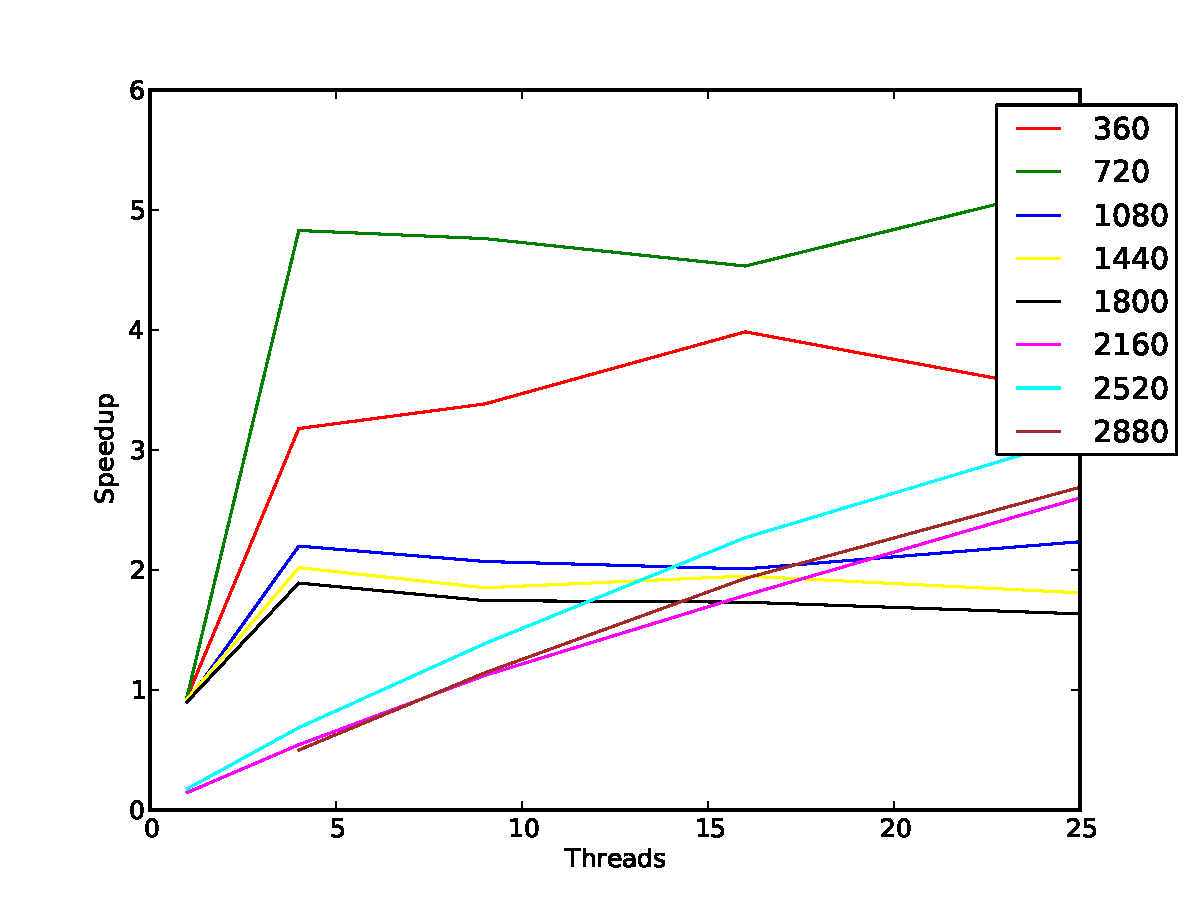
\includegraphics[width=0.5\linewidth]{e5_strong_bindel_baseline.pdf}
\caption{Strong scaling speedup for running on the Xeon E5 2620s. Baseline for calculating speedup is Professor Bindel's code from the point at which we forked it.}
\end{figure}

\begin{figure}[h!]
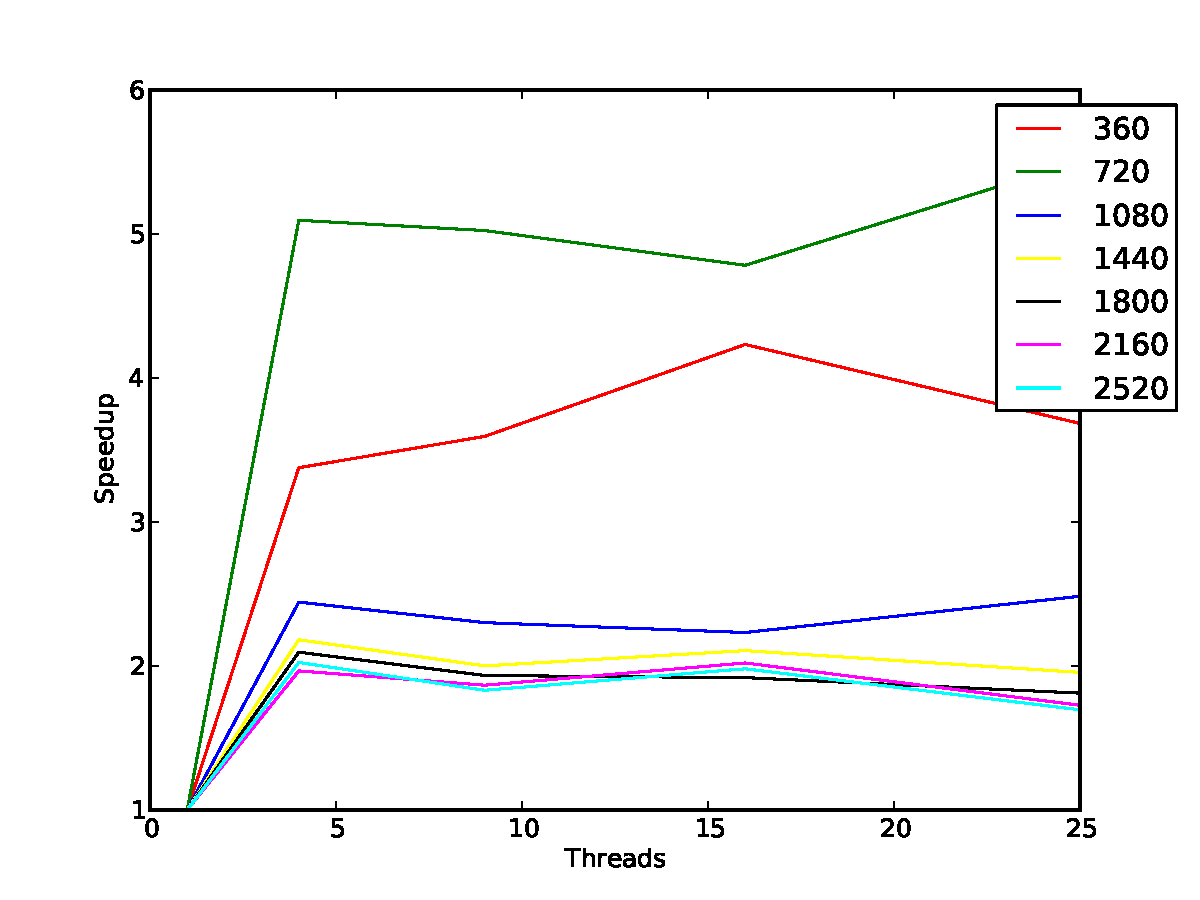
\includegraphics[width=0.5\linewidth]{e5_strong_e5_baseline.pdf}
\caption{Strong scaling speedup for running on the Xeon E5 2620s. Baseline for calculating speedup is our code running a single thread on the main node (Xeon E5 2620s).}
\end{figure}

\subsubsection{Weak Scaling}
\begin{figure}[h!]
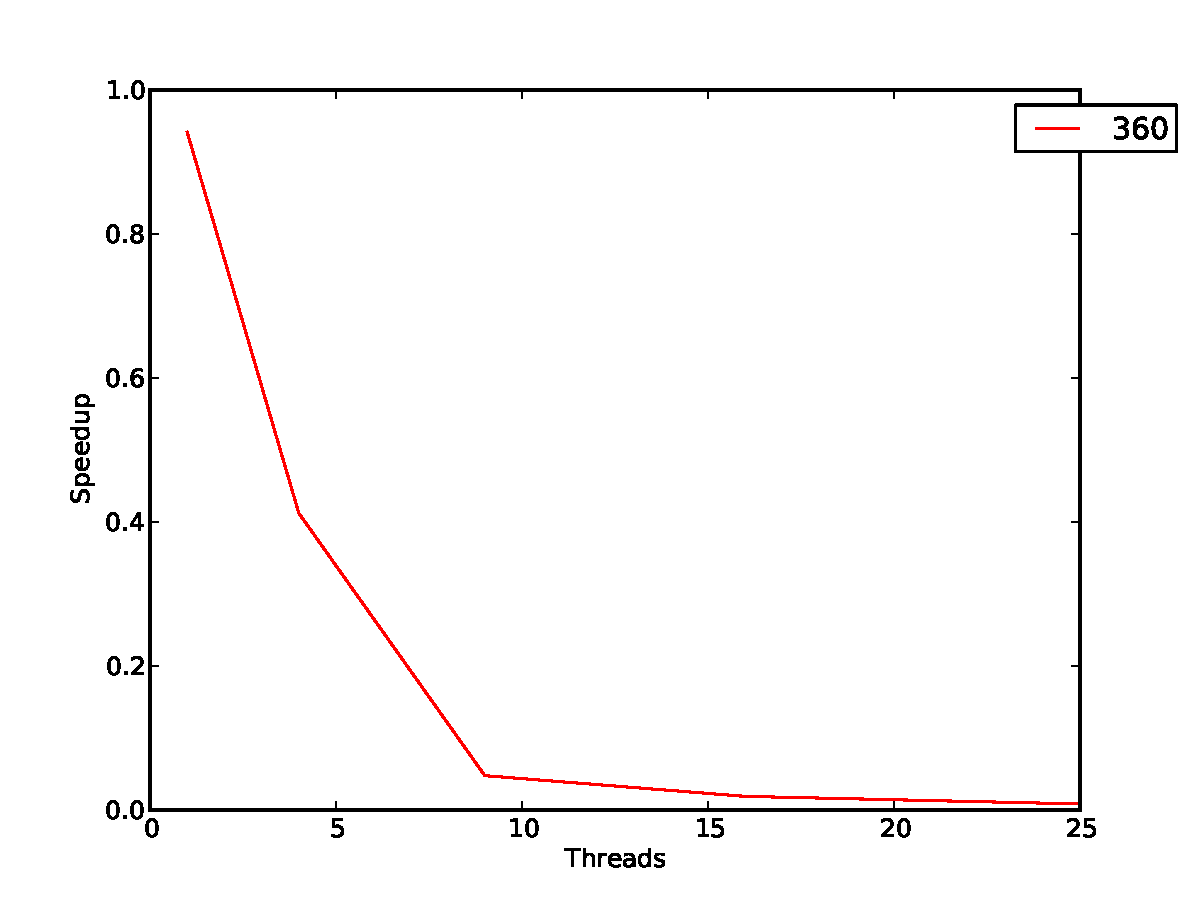
\includegraphics[width=0.5\linewidth]{e5_weak_bindel_baseline.pdf}
\caption{Weak scaling speedup for running on the Xeon E5 2620s. Baseline for calculating speedup is Professor Bindel's code from the point at which we forked it.}
\end{figure}

\begin{figure}[h!]
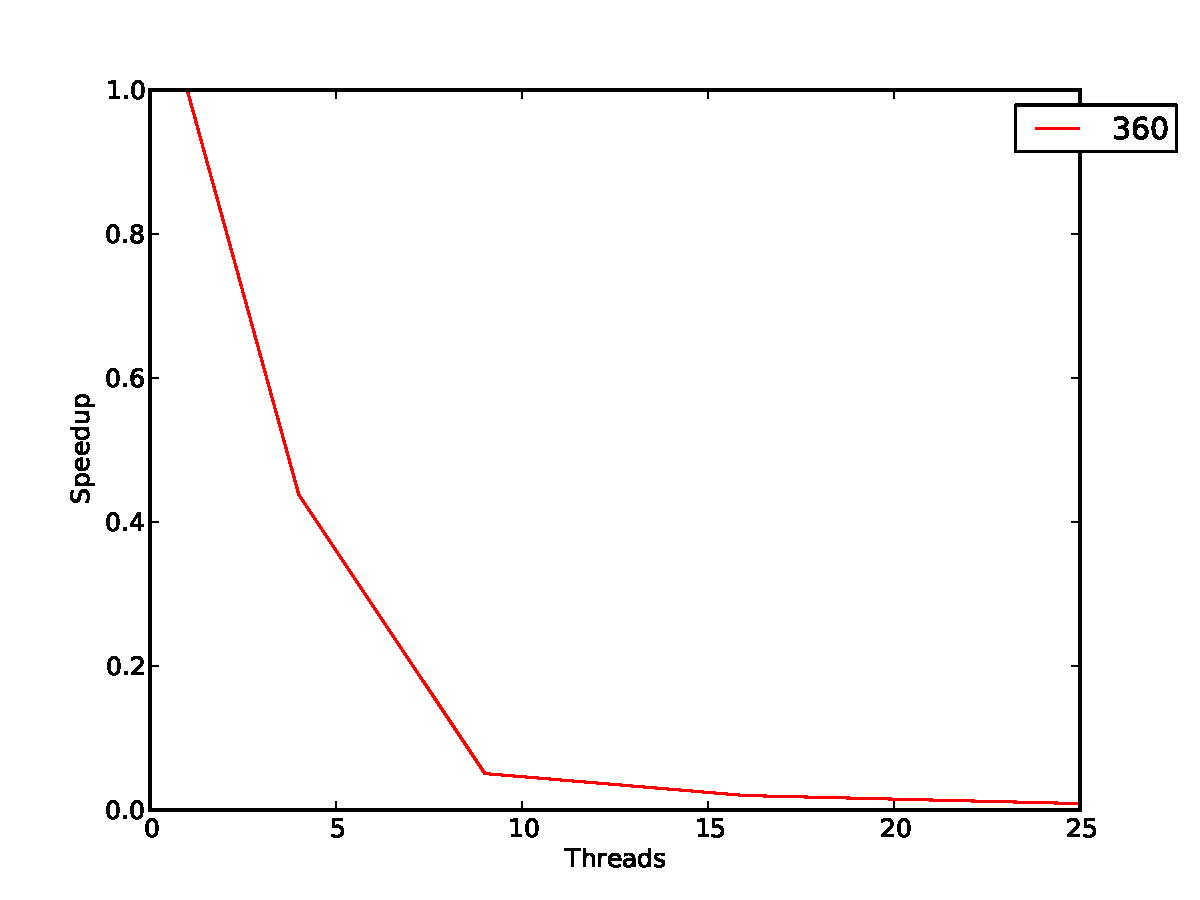
\includegraphics[width=0.5\linewidth]{e5_weak_e5_baseline.pdf}
\caption{Weak scaling speedup for our parallel code running on the Xeon E5 2620s. Baseline for calculating speedup is our code running a single thread on the main node (Xeon E5 2620s).}
\end{figure}

\subsection{Xeon Phi Performance}

\subsubsection{Strong Scaling}
\begin{figure}[h!]
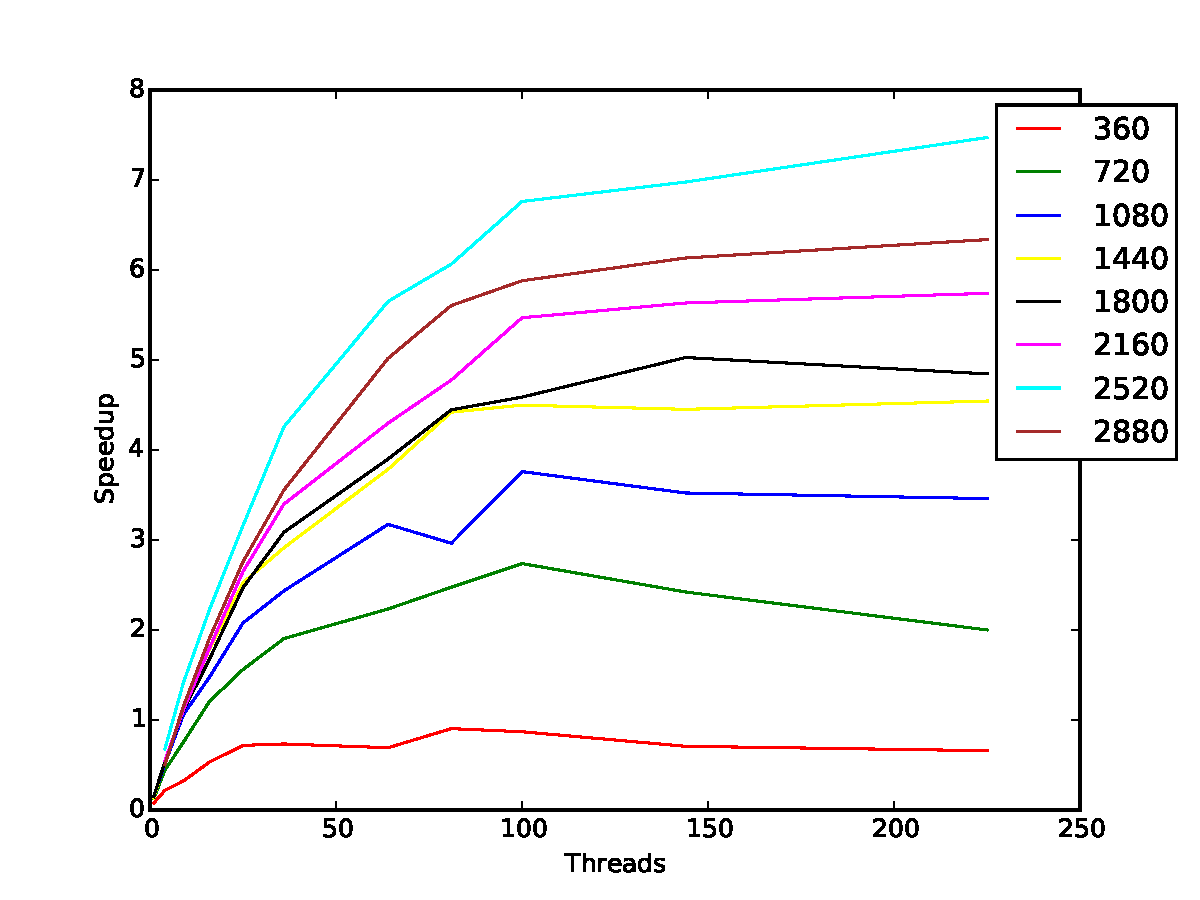
\includegraphics[width=0.5\linewidth]{mic_strong_bindel_baseline.pdf}
\caption{Strong scaling speedup for our offloaded Phi code. Baseline for calculating speedup is Professor Bindel's code from the point at which we forked it.}
\end{figure}

\begin{figure}[h!]
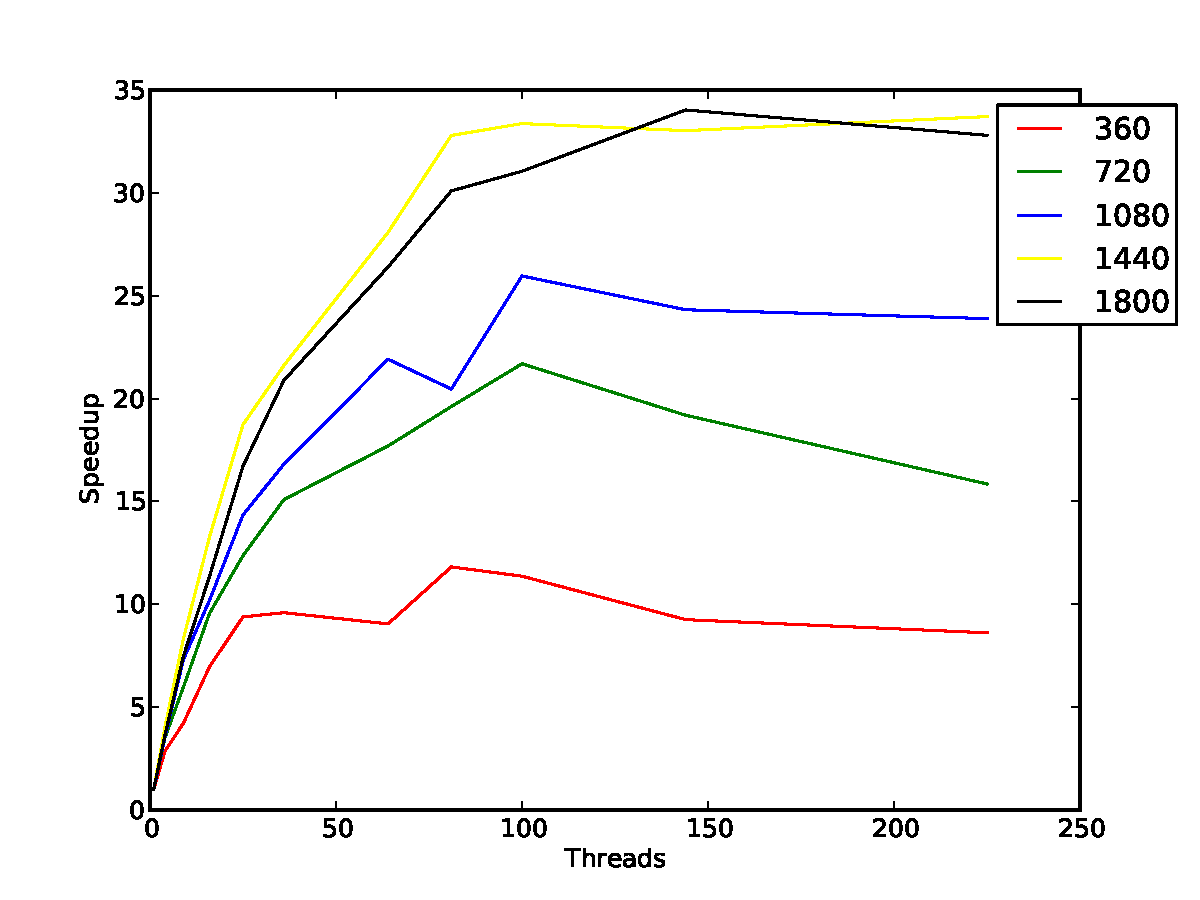
\includegraphics[width=0.5\linewidth]{mic_strong_mic_baseline.pdf}
\caption{Strong scaling speedup for our offloaded Phi code. Baseline for calculating speedup is our code running a single thread offloaded to the Phis.}
\end{figure}

\subsubsection{Weak Scaling}
\begin{figure}[h!]
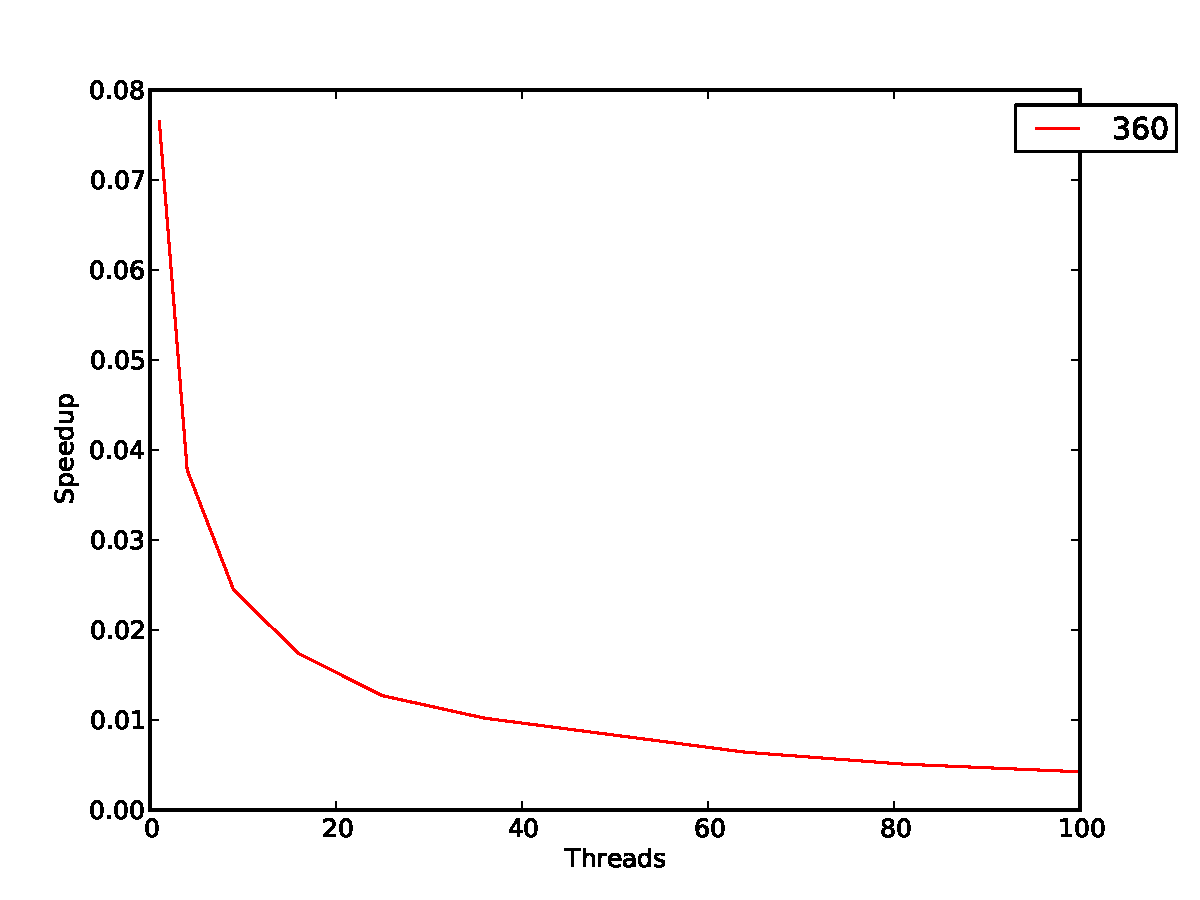
\includegraphics[width=0.5\linewidth]{mic_weak_bindel_baseline.pdf}
\caption{Weak scaling speedup for our offloaded Phi code. Baseline for calculating speedup is Professor Bindel's code from the point at which we forked it.}
\end{figure}

\begin{figure}[h!]
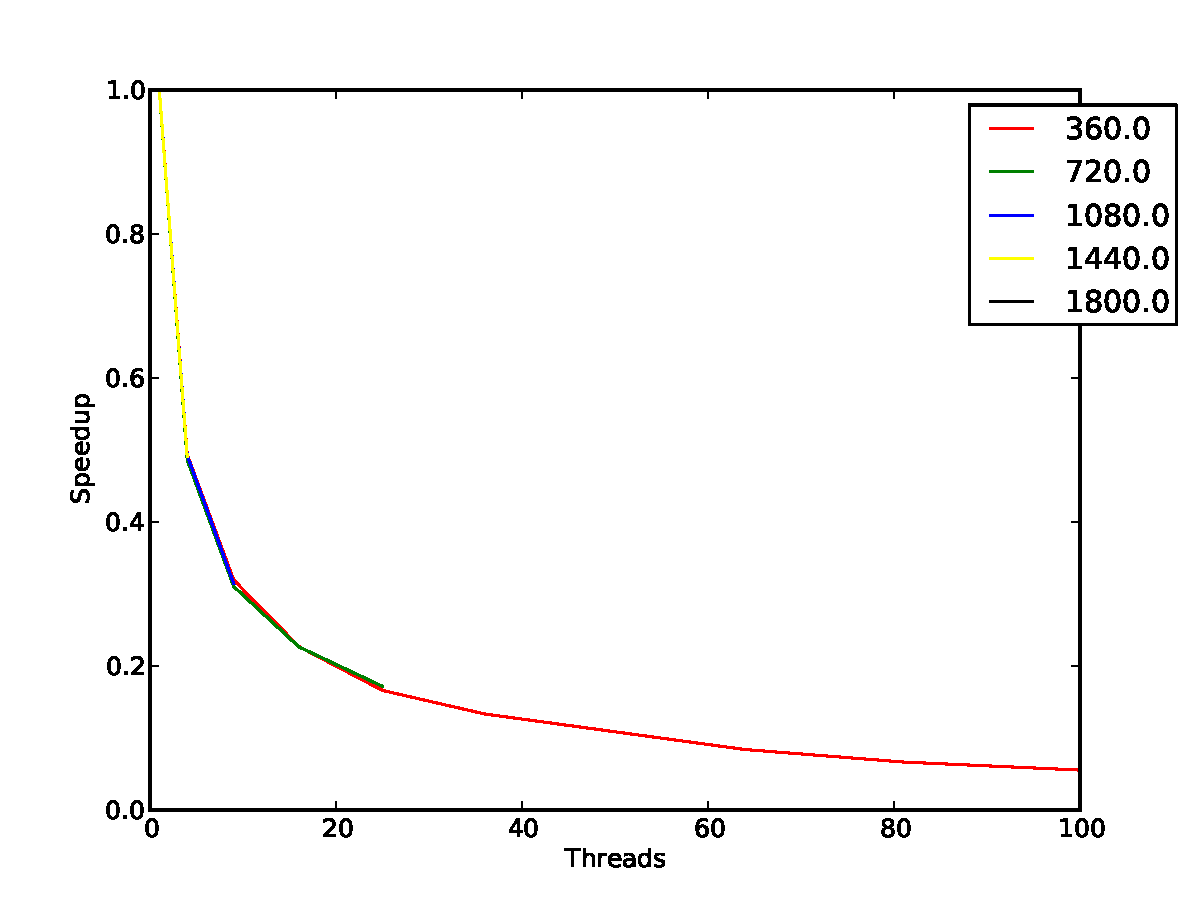
\includegraphics[width=0.5\linewidth]{mic_weak_mic_baseline.pdf}
\caption{Weak scaling speedup for our offloaded Phi code. Baseline for calculating speedup is our code running a single thread offloaded to the Phis.}
\end{figure}

\subsection{Batch size Performance}

We were also interested in how our code performed when we increased batch size on the Xeon Phi boards. We found that when we increased batch size to two rather than 1 (so 4 steps rather than 2 steps), that our total time was actually slightly worse. This is likely because there are few barriers in our code (one after our speed calculation, one after our copy and compute steps calculation, one after our synchronize section) and no single-threaded sections which take large computation time. Thus synchronization wasn't all the expensive and the extra work (in terms of more ghost cells that have to be calculated for) does not outweigh the decreased synchronization frequency.

Furthermore it is likely that because we have to back-off our dt when doing a batch size of moer than 1 in order to be conservative and not violate the CFL constraint we must do more steps total for our simulatino to complete which is more work. Further a larger batch size potentially leads to many extra steps taken near the end of a simulation when a smaller number of steps would suffice.

\begin{figure}[h!]
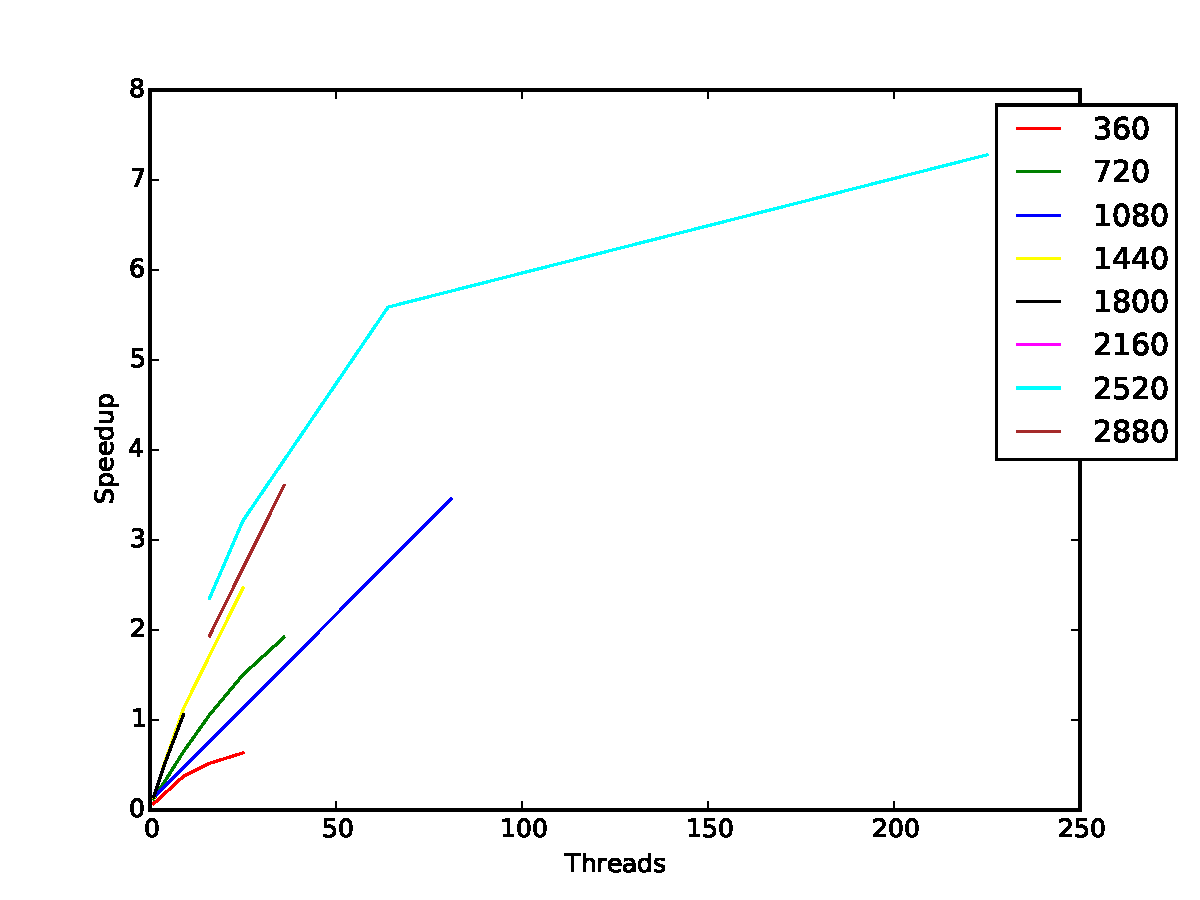
\includegraphics[width=0.5\linewidth]{mic_strong_bindel_baseline_batchsize2.pdf}
\caption{Strong scaling speedup for our offloaded Phi code with a batch size of 2. Baseline for calculating speedup is Professor Bindel's code at the point where we forked it. We can see that speedup is slightly worse than our speedup for batch size of 1.}
\end{figure}

\end{document}















